\documentclass[tikz,border=80pt]{standalone}
\usepackage{tikz}
\usetikzlibrary{scopes}
\usepackage{verbatim}
\usetikzlibrary{calc,angles,patterns,quotes}
\usetikzlibrary{positioning}


\tikzset{
    right angle quadrant/.code={
        \pgfmathsetmacro\quadranta{{1,1,-1,-1}[#1-1]}     % Arrays for selecting quadrant
        \pgfmathsetmacro\quadrantb{{1,-1,-1,1}[#1-1]}},
    right angle quadrant=1, % Make sure it is set, even if not called explicitly
    right angle length/.code={\def\rightanglelength{#1}},   % Length of symbol
    right angle length=1ex, % Make sure it is set...
    right angle symbol/.style n args={3}{
        insert path={
            let \p0 = ($(#1)!(#3)!(#2)$) in     % Intersection
                let \p1 = ($(\p0)!\quadranta*\rightanglelength!(#3)$), % Point on base line
                \p2 = ($(\p0)!\quadrantb*\rightanglelength!(#2)$) in % Point on perpendicular line
                let \p3 = ($(\p1)+(\p2)-(\p0)$) in  % Corner point of symbol
            (\p1) -- (\p3) -- (\p2)
        }
    }
}



\begin{document}

\def\iangle{35} % Angle of the inclined plane
\def\down{-90}
\def\arcr{0.5cm} % Radius of the arc used to indicate angles
\def\ang{30}
\def\radius{5em} % radiaus of a timber
\def\dotsize{0.1em}
\def\nsize{0.5}


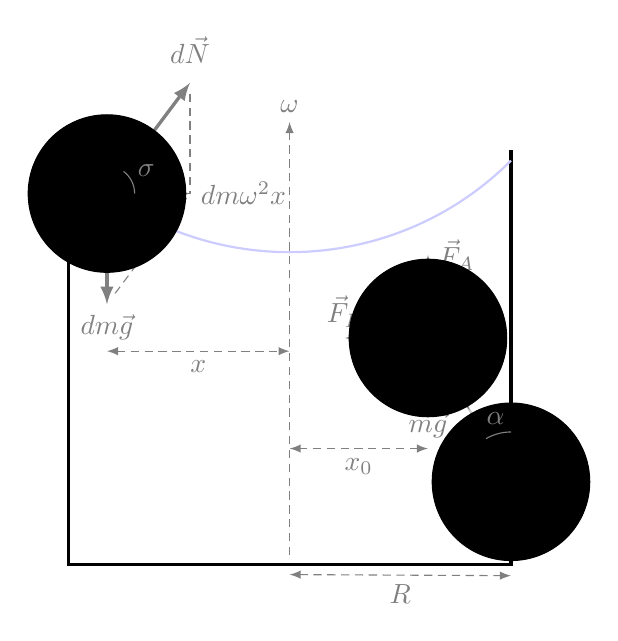
\begin{tikzpicture}[
    force/.style={>=latex, very thick,draw=gray,fill=gray},
    axis/.style={densely dashed,gray},
    M/.style={rectangle,draw,fill=lightgray,minimum size=0.5cm,thin},
    m/.style={rectangle,draw=black,fill=lightgray,minimum size=0.3cm,thin},
    plane/.style={draw=black,fill=blue!10},
    string/.style={draw=red, thick},
    pulley/.style={thick},
    timber-fill/.style={pattern=north west lines, pattern color=brown!50}
]


\node (tank-bottom-middle) {};
\draw [->, >=latex, axis] (tank-bottom-middle) -- ++(0, 16em) node[above] {$\omega$};
\draw [very thick] (tank-bottom-middle.center) -- ++(8em, 0) node(tank-bottom-right) {}
                                               -- ++ (0, 15em)
                                               node[pos=0.2] (tank-attach-right) {}
                                               node (tank-top-right) {};


\draw[thick, gray!40] (tank-attach-right.center) -- ++(120:5em) node [midway, below] (rope-length-label){} 
                                                                node (balloon-rope) {};

\node[gray] at (rope-length-label.south) {$l$};

\draw[fill] (tank-attach-right.center) circle(\dotsize);

\path (balloon-rope.center) -- ++(120:1em) node (balloon-center){};

\draw [red] (balloon-center.center) circle(1em);



\draw [very thick] (tank-bottom-middle.center) -- ++(-8em, 0) node(tank-bottom-left) {} 
                                               -- ++ (0, 15em) node (tank-top-left) {};

\draw [thick, blue!20] (tank-top-left.south) to[bend right=45] 
      node[pos=0.1] (water-surface-parcel) {} 
      node[midway] (water-surface-middle) {} (tank-top-right.south);

\draw [>=latex,<->, axis] (tank-bottom-middle.south) -- node[midway, below] {$R$} (tank-bottom-right.south);


% draw the forces on the balloon
\draw[->, force] (balloon-center.center) -- ++(0, -2.3em) node [below,gray] (balloon-glabel) {$m\vec{g}$};
\draw[->, force] (balloon-center.center) -- ++(0, 3em) node [right,gray] {$\vec{F}_{A}$};
\draw[->, force] (balloon-center.center) -- ++(-60:3em) node [right=0.2em,pos=0.4,gray] {$\vec{T}$};
\draw[->, force] (balloon-center.center) -- ++(-180:3em) node [above,gray] {$\vec{F}_{P}$};


% draw the forces on the water element
\draw[->, force] (water-surface-parcel.center) -- ++(0, -4em) node (gtip) {}  
                                                              node [below,gray] (parcel-glabel) {$dm\vec{g}$};

\draw[->, force] (water-surface-parcel.center) -- ++(3em, 0) node (nettip) {}
                                                             node [right, gray] {$dm\omega^2 x $};

\draw[->, force] (water-surface-parcel.center) -- ++(3em, 4em) node (ntip) {} 
                                                               node [above=0.3em,gray] {$d\vec{N} $};

\draw[axis] (ntip) -- (nettip.center);
\draw[axis] (gtip) -- (nettip.center);

% show distance x
\draw [>=latex,<->, axis] (parcel-glabel.south) -- 
                          ($(tank-bottom-middle.center)!(parcel-glabel.south)!(water-surface-middle.center)$)
                          node[midway, below]{$x$};

% show distance x0
\draw [>=latex,<->, axis] (balloon-glabel.south) -- 
                          ($(tank-bottom-middle.center)!(balloon-glabel.south)!(water-surface-middle.center)$)
                          node[midway, below]{$x_0$};


% mark the center of the balloon
\draw[fill] (balloon-center.center) circle(\dotsize); 
\draw[fill] (water-surface-parcel.center) circle(\dotsize);


% mark angles
\draw[gray] pic ["$\sigma$", 
                 draw=gray, 
                 angle eccentricity=1.2, 
                 angle radius=1em,
                 pic text options={shift={(0.35em,0.3em)}}]{angle=nettip--water-surface-parcel--ntip};
                 
\draw[gray] pic ["$\alpha$", 
                 draw=gray, 
                 angle eccentricity=1.2, 
                 angle radius=1.8em,
                 pic text options={shift={(0, 0.2em)}}]{
                    angle=tank-top-right--tank-attach-right--balloon-center};

\end{tikzpicture}



\end{document}
